\documentclass{article}
\usepackage[final]{neurips_2024}

\usepackage[utf8]{inputenc} % allow utf-8 input
\usepackage[T1]{fontenc}    % use 8-bit T1 fonts
\usepackage{hyperref}       % hyperlinks
\usepackage{url}            % simple URL typesetting
\usepackage{booktabs}       % professional-quality tables
\usepackage{amsfonts}       % blackboard math symbols
\usepackage{nicefrac}       % compact symbols for 1/2, etc.
\usepackage{microtype}      % microtypography
\usepackage{xcolor}         % colors

\usepackage{graphicx}
\usepackage{float}

\title{Homework 5}

\author{
  Kevin Lei \\
  Department of Computer Science and Engineering \\
  Texas A\&M University \\
  College Station, TX 77843 \\
  \texttt{kevinlei@tamu.edu} \\
}

\begin{document}
\maketitle

\section{Part A}

For feature set \textit{i}, the network achieved an accuracy of 0.5.

\begin{figure}[H]
  \centering
  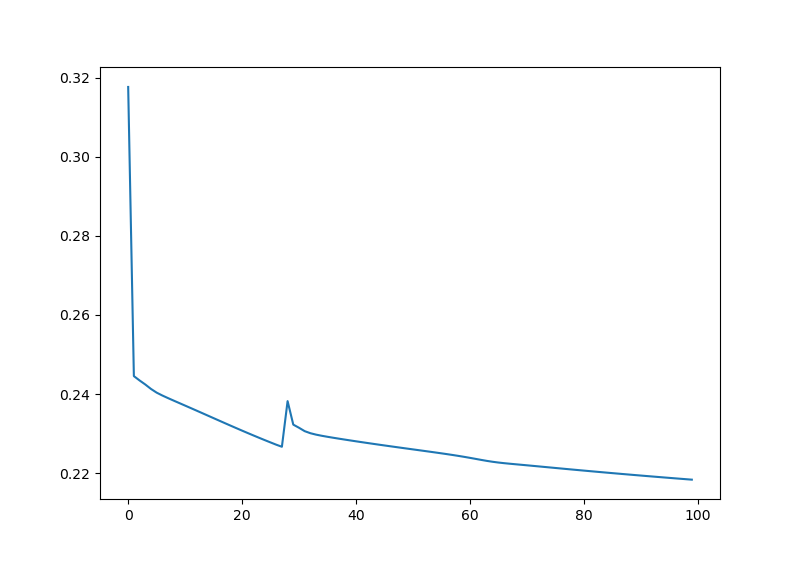
\includegraphics[width=0.8\textwidth]{Figure_1.png}
  \caption{Cost vs Epoch for Feature Set \textit{i}}
\end{figure}

Feature set \textit{ii} achieved an accuracy of 1.0, and the cost vs epoch plot is shown below.

\begin{figure}[H]
  \centering
  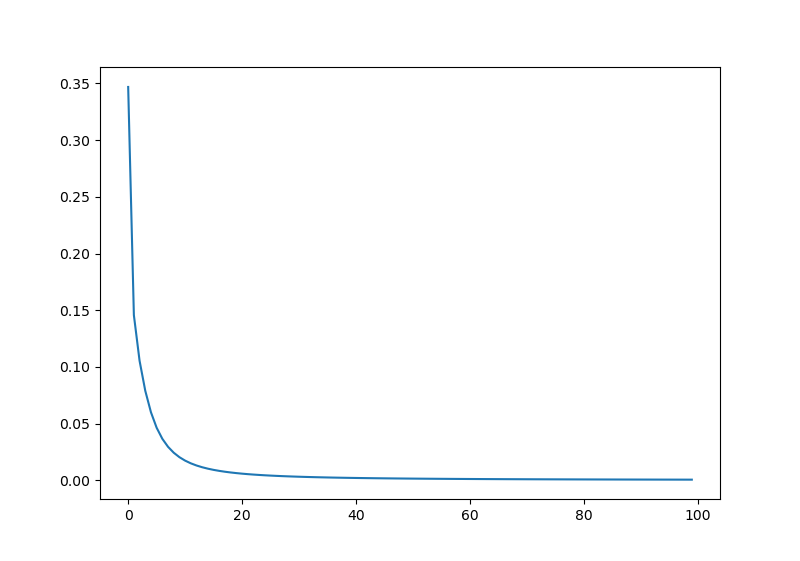
\includegraphics[width=0.8\textwidth]{Figure_2.png}
  \caption{Cost vs Epoch for Feature Set \textit{ii}}
\end{figure}

Obviously, there are some differences in results for the two data sets even though our network is the same.
From figure 1, we can see that the cost sharply decreases at the beginning and has a small spike later.
Compare this to figure 2, where the cost decreases smoothly and levels off near 0.
This may indicate that the network needs more epochs to converge for feature set \textit{i}.
Increasing the number of epochs to 10000 lead to an interesting cost plot for feature set \textit{i}:

\begin{figure}[H]
  \centering
  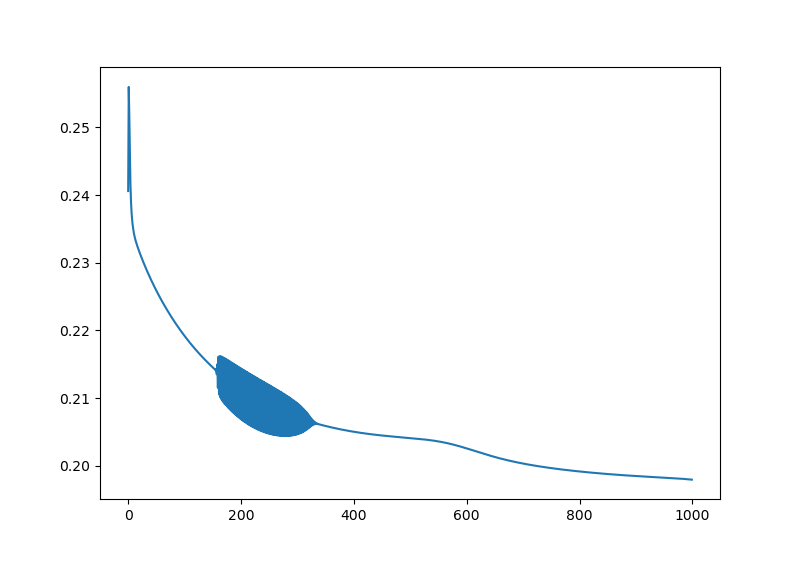
\includegraphics[width=0.8\textwidth]{Figure_3.png}
  \caption{Cost vs Epoch for Feature Set \textit{i} with 10000 epochs}
\end{figure}

It seems that the cost oscillates wildly at around 200 epochs, and reaches a final loss of around 0.20 at the end.
The accuracy is now higher at 0.73, but still not as good as feature set \textit{ii}.
We can solve this issue by trying to tweak other network parameters, such as the learning rate, number of hidden layers, or number of neurons in each layer.

\section{Part B}

Increasing the number of neurons should generally allow neural networks to learn more complex functions, aka increaing the capacity of the network.
Theoretically, this means that if feature set \textit{i} is not linearly separable, increasing the number of neurons should allow the network to learn the function better.
In practice, increasing the number of neurons from 5 to 20 did not improve the accuracy of the network for feature set \textit{i}.
The accuracy remained at 0.5, and the cost vs epoch plot is shown below.

\begin{figure}[H]
  \centering
  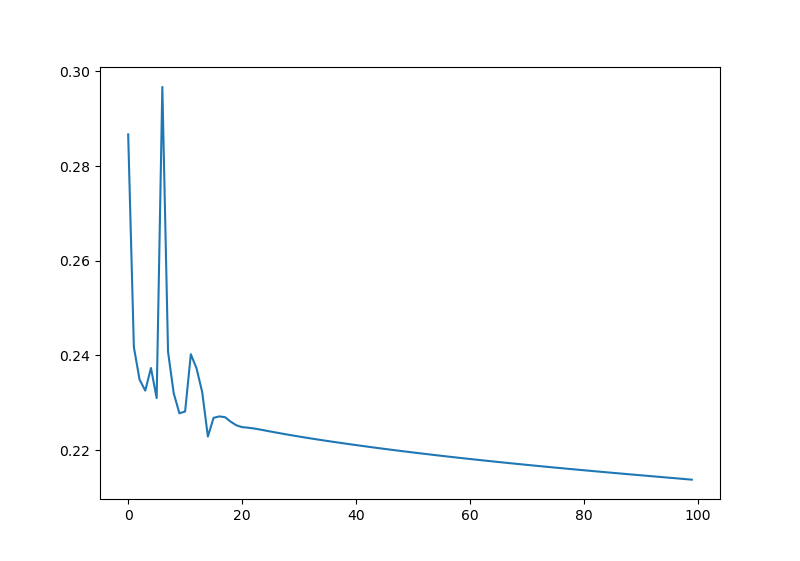
\includegraphics[width=0.8\textwidth]{Figure_4.png}
  \caption{Cost vs Epoch for Feature Set \textit{i} with 20 neurons}
\end{figure}

The cost plot is similar to the one with 5 neurons, but with more variability in the beginning. 
For feature set \textit{ii}, the accuracy remained at 1.0, and the cost vs epoch plot is shown below.

\begin{figure}[H]
  \centering
  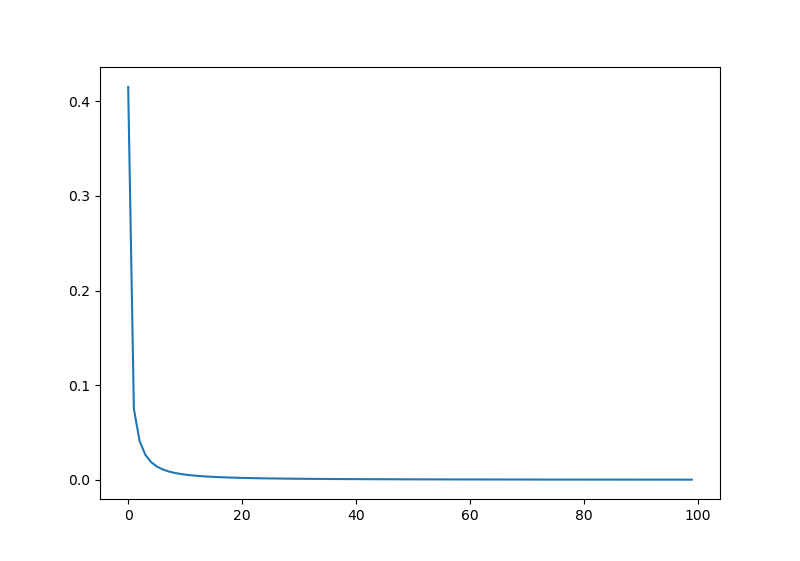
\includegraphics[width=0.8\textwidth]{Figure_5.png}
  \caption{Cost vs Epoch for Feature Set \textit{ii} with 20 neurons}
\end{figure}

\section{Part C}

Adding a hidden layer to the network should also allow the network to learn more complex functions.
Adding one more hidden layer improved the accuracy of the network for feature set \textit{i} to 0.55, which is slightly better but still not great.
The cost vs epoch plot is shown below.

\begin{figure}[H]
  \centering
  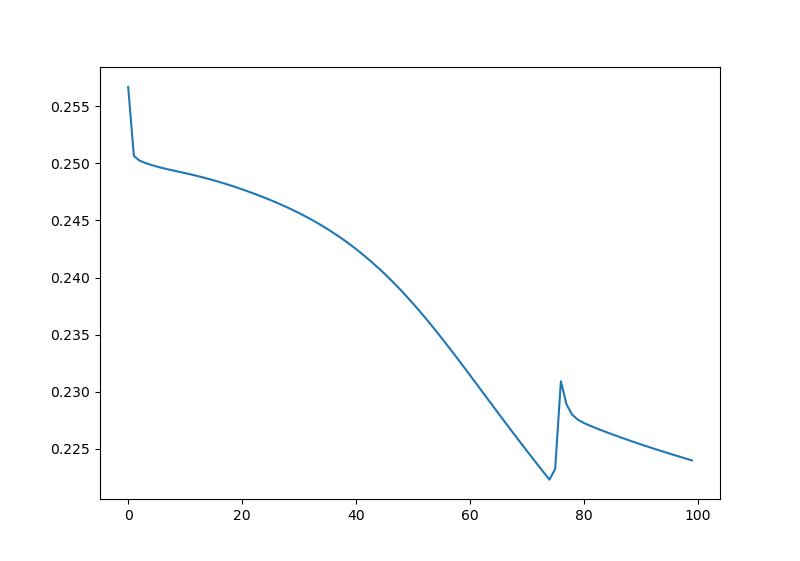
\includegraphics[width=0.8\textwidth]{Figure_6.png}
  \caption{Cost vs Epoch for Feature Set \textit{i} with 2 hidden layers}
\end{figure}

Here we see that the cost decreases slower and has the same spike as before.

For feature set \textit{ii}, the accuracy remained at 1.0, and the cost vs epoch plot is shown below.

\begin{figure}[H]
  \centering
  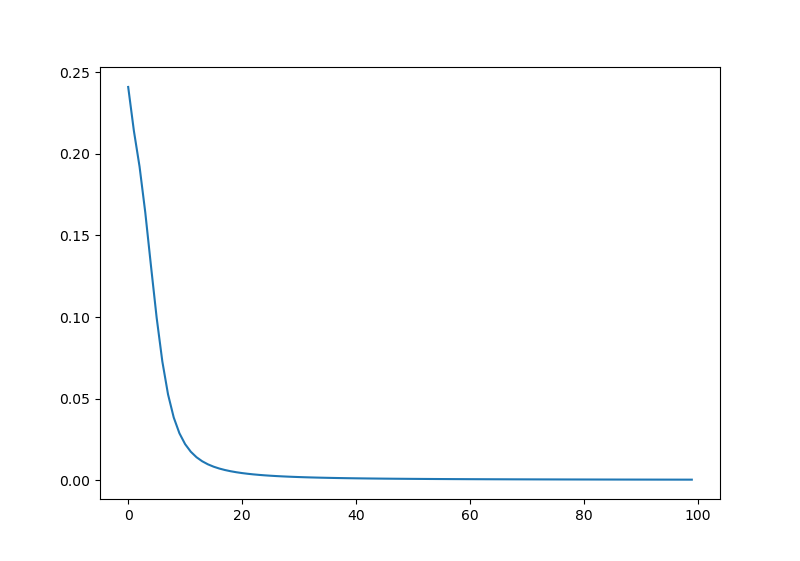
\includegraphics[width=0.8\textwidth]{Figure_7.png}
  \caption{Cost vs Epoch for Feature Set \textit{ii} with 2 hidden layers}
\end{figure}

In the end NET1 and NET3 did not perform all that much different for feature set \textit{i} and exactly the same for feature set \textit{ii}.

\section{Part D}
Using more input features is another way we can try to increase the accuracy of the network.
Here we use all 4 features for training and inference.
Now, the accuracy for feature set \textit{i} is 0.95, a significant improvement over the previous results.
The cost vs epoch plot is shown below.

\begin{figure}[H]
  \centering
  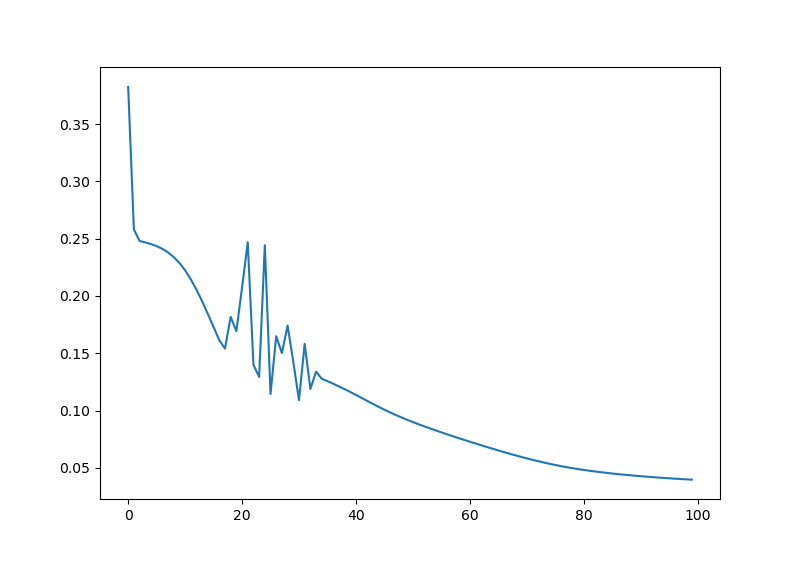
\includegraphics[width=0.8\textwidth]{Figure_8.png}
  \caption{Cost vs Epoch for Feature Set \textit{i} with all features}
\end{figure}

For feature set \textit{ii}, the accuracy remained at 1.0, and the cost vs epoch plot is shown below.

\begin{figure}[H]
  \centering
  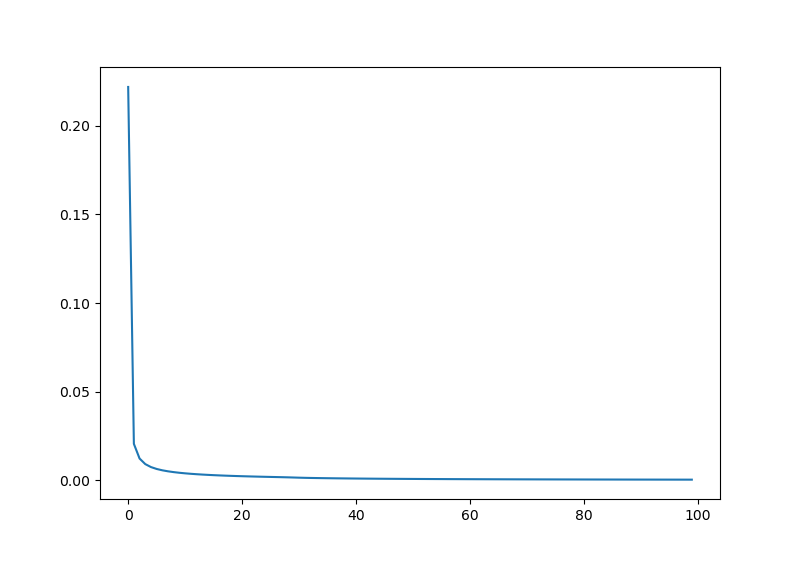
\includegraphics[width=0.8\textwidth]{Figure_9.png}
  \caption{Cost vs Epoch for Feature Set \textit{ii} with all features}
\end{figure}

Using all four features provides a solution for the accuracy issue with feature set \textit{i}.
NET4 performed the best out of all the networks for feature set \textit{i}.

\end{document}